\anonsection{Условие лабораторной работы}
Необходимо промоделировать систему, состоящую из генератора, памяти, и обслуживающего аппарата. Генератор подает сообщения, распределенные по равномерному закону, они приходят в память и выбираются на обработку по закону из ЛР1. Количество заявок конечно и задано. Предусмотреть случай, когда обработанная заявка возвращается обратно в очередь. Необходимо определить оптимальную длину очереди, при которой не будет потерянных сообщений. Реализовать с использованием GPSS.

Мой вариант -- 4.
Согласно требованиям к лабораторной работе, нужно провести работу с двумя распределениями:
\begin{enumerate}
	\item Равномерное распределение.
	\item Распределение Эрланга.
\end{enumerate}

\anonsection{Теоретическая часть}
В этом разделе будет дано описание распределений, использованных в лабораторной работе, а также подходов к решению задачи.

\subsection*{Равномерное распределение}
\textbf{Равномерное распределение} -- распределение случайной величины, принимающей значения, принадлежащие некоторому промежутку конечной длины, характеризующееся тем, что плотность вероятности на этом промежутке постоянна.


\subsubsection*{Вывод основных формул}
Пусть $A$ и $B$ -- границы промежутка равномерного распределения. Исходя из определения, плотность можно посчитать по формуле \ref{dens}:
\begin{equation}
	\label{dens}
	f(x)= 
	\begin{cases}
		C,& \text{если } x \in [A, B]\\
		0,              & \text{иначе}
	\end{cases}
\end{equation}

Одно из важнейших свойств плотности распределения -- нормированность. Его математическое представление выражено формуле \ref{prop}:
\begin{equation}
	\label{prop}
	\int_{-\infty}^{\infty} f(x) \,dx \ = 1
\end{equation}

Для равномерного распределения вычислим интеграл, учитывая свойства интеграла и формулу \ref{dens}:
\begin{equation}
	\label{viv}
	\int_{-\infty}^{\infty} f(x) \,dx \ = \int_{-\infty}^{A} 0 \,dx \ + \int_{A}^{B} C \,dx \ + \int_{B}^{\infty} 0 \,dx \ = \int_{A}^{B} C \,dx \ = C*(B - A)
\end{equation}

Вычислим плотность распределения, сравняв полученное в формулах \ref{prop} и \ref{viv}:
\begin{equation}
	\label{vivProb}
	C*(B - A) = 1 \rightarrow C = 1 / (B - A)
\end{equation}

Окончательная формула плотности распределения для равномерной случайной величины представлена на формуле \ref{dens1}:
\begin{equation}
	\label{dens1}
	f(x)= 
	\begin{cases}
		1 / (B - A),& \text{если } x \in [A, B]\\
		0,              & \text{иначе}
	\end{cases}
\end{equation}

Функцию распределения, зная плотность, можно рассчитать по формуле \ref{func}:
\begin{equation}
	\label{func}
	F_X(x) = \int_{-\infty}^{x} f_X(t) \,dt \ = 1
\end{equation}

\newpage
Для равномерного распределения требуется рассмотреть три случая: $x < A$; $x \in [A, B]$; $x > B$. Рассчитывая интеграл для каждого из трёх случаев, получим формулу \ref{funcRes}:
\begin{equation}
	\label{funcRes}
	F_X(x)= 
	\begin{cases}
		0 & \text{если } x < A\\
		\frac{x - A}{B - A},& \text{если } x \in [A, B]\\
		1,              & x > B
	\end{cases}
\end{equation}

\subsection*{Распределение Эрланга}
\textbf{Распределение Эрланга} -- частный случай Гамма-распределения, двухпараметрическое абсолютно непрерывное распределение, в котором параметр $k$ принимает целочисленное значение.

\subsubsection*{Основные формулы}
Распределение Эрланга задаётся двумя параметрами: $\alpha > 0$ и $k > 0$, причём второй параметр обязательно должен быть целым числом. 

Формула плотности вероятности случайной величины, распределённой по закону Эрланга, представлена на формуле \ref{probEr}:
\begin{equation}
	\label{probEr}
	f(x)= 
	\begin{cases}
		\frac{\alpha  (\alpha*x)^{k - 1}} {(k - 1)!}e^{-\alpha*x} & \text{если } x \geq 0 \\
		0,              & x < 0
	\end{cases}
\end{equation}

Функция распределения случайной величины выражена формулой \ref{funcEr}:
\begin{equation}
	\label{funcEr}
	F(x)= 
	\begin{cases}
		\frac{\int_{0}^{x} t^{k-1}*e^{-x/\alpha} \,dt \ } {(k - 1)!*\alpha^k} & \text{если } x \geq 0 \\
		0,              & x < 0
	\end{cases}
\end{equation}

\newpage

\anonsection{Реализация}
В этом разделе будет приведены листинги кода реализации алгоритмов, продемонстрирована работа программы и построены таблицы с результатами.

\subsection*{Листинги кода}
Для реализации ПО был использован язык GPSS

На рисунке 1 представлен код программы.

На рисунке 2 представлен отчет работы программы при 1000 заявках с параметрами $A=0$. $B=2$ для равномерного распределения,
$k=1, \alpha=1$ для распределения Эрланга. 

\FloatBarrier
\begin{figure}[h]	
	\begin{center}
		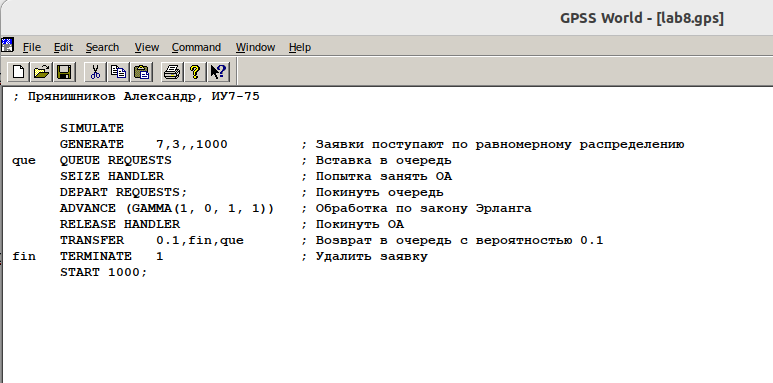
\includegraphics[width=\linewidth]{inc/png/code.png}
	\end{center}
	\captionsetup{justification=centering}
	\caption{Код программы}
\end{figure}
\FloatBarrier

\FloatBarrier
\begin{figure}[h]	
	\begin{center}
		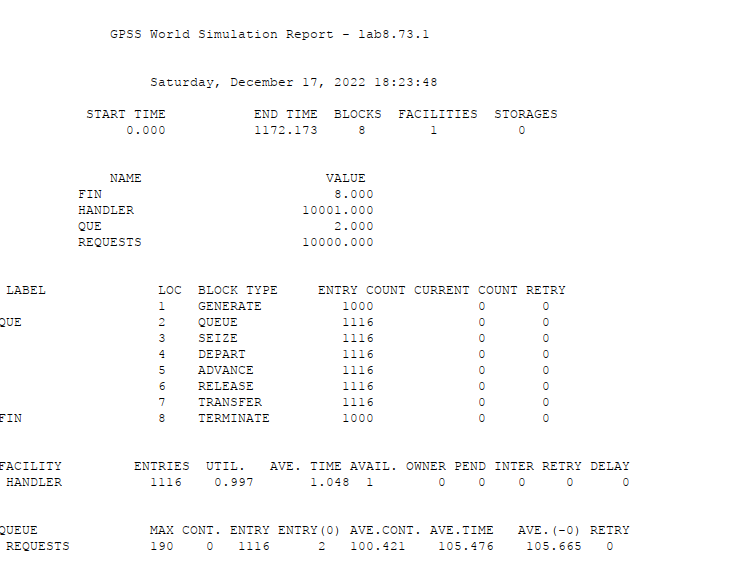
\includegraphics[width=\linewidth]{inc/png/report.png}
	\end{center}
	\captionsetup{justification=centering}
	\caption{Отчет работы программы}
\end{figure}
\FloatBarrier


\subsection*{Полученные результаты}
Тестирование проводилось при различных параметрах вероятности $p$ возврата обработанной заявки в очередь. 
Результаты для $p = 0.1$ приведены в таблице 1.
Результаты для $p = 0.5$ приведены в таблице 2.
Для обоих таблиц: первый столбец -- количество обработанных заявок, во втором столбце -- параметры равномерного распределения, в третьем -- параметры распределения Эрланга.

\FloatBarrier
\begin{table}[h]
	\caption{Таблица полученных значений при $ p = 0.1 $}
	\centering
	\begin{tabular}{ | l | l | l | l |}
		\hline
		N заявок & A, B & K, $\alpha$ & Результат \\
		\hline
		1000 & 1, 5 & 1, 1 & 3 \\
		\hline
		1000 & 0, 2 & 1, 1 & 190  \\
		\hline
		1000 & 0, 10 & 1, 1 & 4  \\
		\hline
		1000 & 1, 5 & 1, 3 & 109 \\
		\hline
	\end{tabular}
\end{table}
\FloatBarrier

\FloatBarrier
\begin{table}[h]
	\caption{Таблица полученных значений при $ p = 0.5 $}
	\centering
	\begin{tabular}{ | l | l | l | l |}
		\hline
		N заявок & A, B & K, $\alpha$ & Результат \\
		\hline
		1000 & 1, 5 & 1, 1 & 6 \\
		\hline
		1000 & 0, 2 & 1, 1 & 570  \\
		\hline
		1000 & 0, 10 & 1, 1 & 5  \\
		\hline
		1000 & 1, 5 & 1, 3 & 514 \\
		\hline
	\end{tabular}
\end{table}
\FloatBarrier